\chapter{Analyse}
\section{Risiken}
Die vierte industrielle Revolution, das \ac{IIoT} und dessen Vielzahl an aktiven und passiven Elementen stellen in ihrer Komplexität eine große Herausforderung für die IT-Sicherheit dar. Einerseits muss die Sicherheit der laufenden Software, der Infrastruktur, Anwendungs- und Rechnersysteme gewährleistet werden, andererseits muss die Betriebssicherheit der Geräte und Anlagen, welche mit dem Internet verbunden sind sichergestellt werden. Das Management der IT-Sicherheit in Industrie 4.0 Netzen geht über Unternehmensgrenzen hinweg, da Netze und Systeme für Kunden, Lieferanden und Partner bereitgestellt werden \cite{DTAG2016}. Somit hat sich auch die Bedrohungslage der Netze geändert. Das \ac{BSI} beschreibt die Top 10 Bedrohungen und deren Folgen für \ac{ICS} \cite{ICSSec2016}.

\begin{enumerate}
    \item Social Engineering und Phishing - 
    \item Einschleusen von Schadsoftware über Wechseldatenträger und externe Hardware - 
    \item Infektion mit Schadsoftware über Internet und Intranet - 
    \item Einbruch über Fernwartungszugänge - 
    \item Menschliches Fehlverhalten und Sabotage - 
    \item Internet-verbundene Steuerungskomponenten - 
    \item Technisches Fehlverhalten und höhere Gewalt - 
    \item Kompromittierung von Extranet und Cloud Komponenten - 
    \item \ac{DoS} und \ac{DDoS} - 
    \item Kompromittierung von Smartphones im Produktionsumfeld - 
\end{enumerate}

TODO - ref. nach BSI
TODO - Bedrohungsanalyse

Um die in \autoref{Grundlagen:Grundprinzipien der sicheren Kommunikation} genannten Schutzziele umzusetzen, ist es notwendig einen größtmöglichen Schutz gegen diese Bedrohungen bereitzustellen. Dafür müssen die Netzwerkinfrastruktur, Integrationsansätze und die eigentliche Kommunikation über die genutzten Protokolle gesichert werden. Dies geschieht u.a. durch die Abschottung von Systemen, die Einschränkung von Zugangsberechtigungen, die Härtung der Sicherheit der genutzten Komponenten, den Einsatz von Verschlüsselungsverfahren und die Schulung der Mitarbeiter um ein Sicherheitsbewusstsein zu schaffen und die Einhaltung von Sicherheitsrichtlinien zu gewährleisten.

\section{Netzwerkinfrastruktur}
TODO - heterogene Netze machen Probleme - Globale Netze haben Latenz, Paketverlust, usw.; müssen Anforderungen gerecht werden.

\subsection{Übertragungsmedium}
Als Übertragungsmedien können neben der klassischen Kabelverbindung auch andere (instabile) Kanäle wie Mobilfunk oder Satelliten in Frage kommen. Um die Kommunikation über alle Medien sicher und zuverlässig zu gestalten, müssen auf technischer Ebene Protokolle genutzt werden, welche es ermöglichen die gegebenen Schutzziele zu realisieren und die Integrität der Daten bei der Übertragung über große Entfernungen zu gewährleisten.

TODO - Übertragungsdistanz - Latenz - Jitter - usw.

\subsection{Defense in Depth Strategie}
Die Norm IEC 62443 - TODO ref. - beschreibt ein Defense in Depth Konzept, um die IT-Sicherheit der Anlagen, die Netzwerksicherheit und Systemintegrität nach dem Stand der Technik zu schützen. Sie gliedert eine Unternehmensinfrastruktur in multiple und redundante Sicherheitsschichten (Zonen), um ein höchstmögliches Sicherheitsniveau zu erreichen. Die unabhängigen Verteidigungslinien sollen Angriffe verzögern, um Zeit für Gegenmaßnahmen zu gewinnen.

Die Kommunikation erfolgt in separierten Netzsegmenten, welche zusätzlich mit \ac{IDS} nutzen, um Angriffe schnell zu erfassen und Gegenmaßnahmen einleiten zu können. Somit wird der Aufwand, um die Shop-Floor-Ebene zu kompromittieren durch den Einsatz von \ac{DMZ}, \ac{IDS}, Paketfilter und Time Access Control wesentlich erhöht. Zusätzlich ist das "`Zone and Conduit"' Modell eines der zentralen Elemente der Defense in Depth Strategie. Die verschiedenen Zonen können nur mittels spezieller Leitungen (Conduits) miteinander kommunizieren.  

\begin{figure}[h]
    \centering
    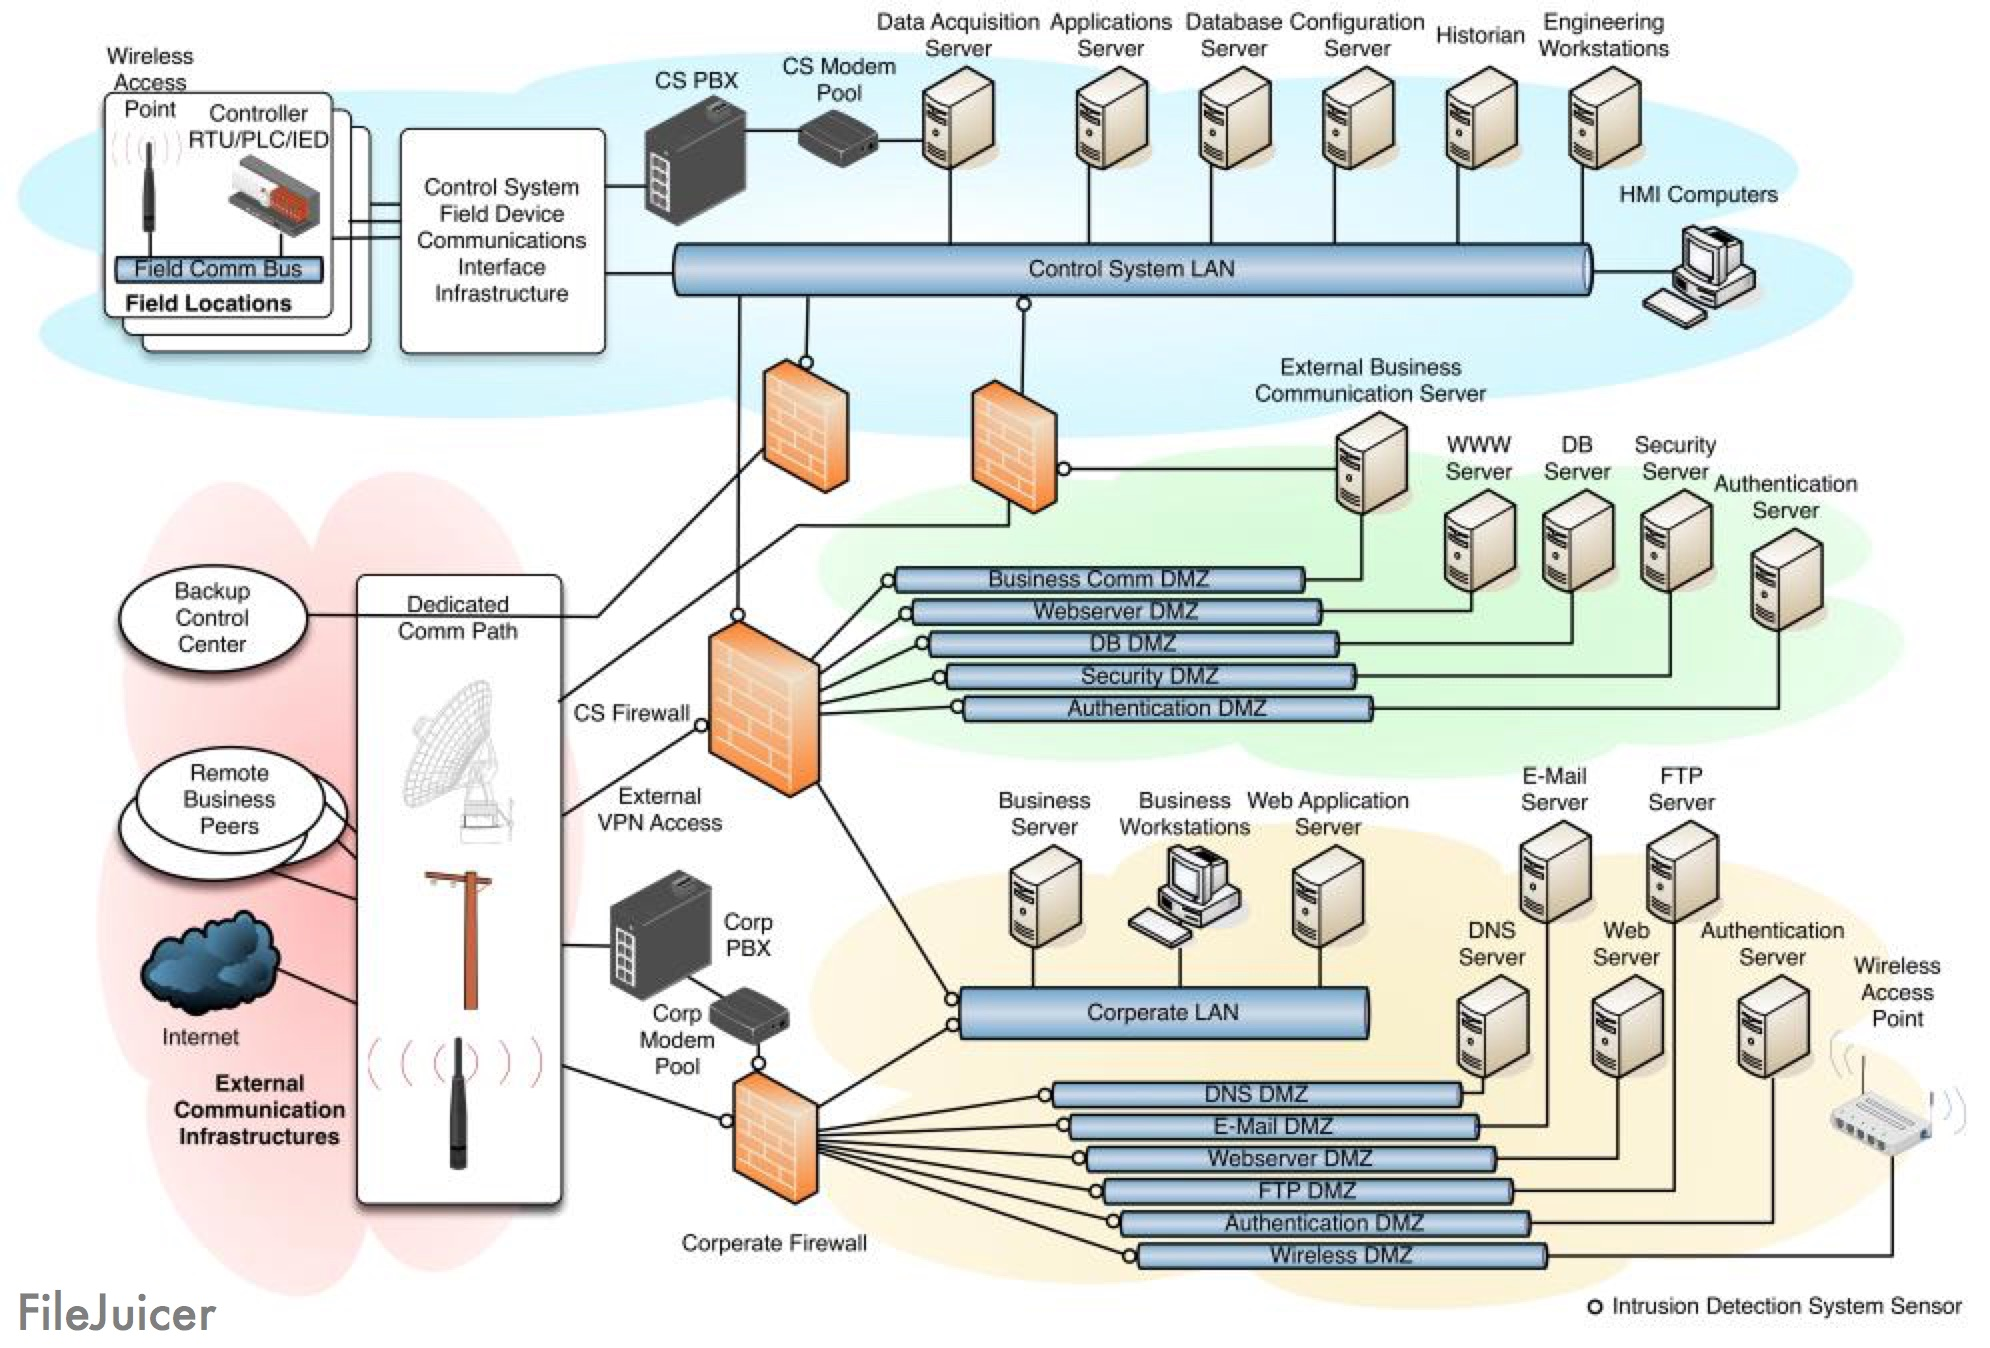
\includegraphics[width=15cm]{defense-in-depth-strategie}
    \caption{Defense in Depth Strategie - \cite{kuipers2006}}
    \label{Kap3:Defense-in-Depth}
\end{figure}

\clearpage

Das Defense in Depth Konzept stellt ein Konzept dar, um Industrieanlagen und Unternehmensnetzwerke vor Angriffen zu schützen. Bei der sich ständig ändernden Bedrohungslage in den komplexen Netzen wird bei dieser Strategie jedoch weniger ein vollständiger Schutz bereitgestellt, als eine Strategie zur Schadensbegrenzung im Falle eines Angriffs.

\section{Integrationsansätze}
Die Grundlage der Industrie 4.0 Kommunikation ist ein standardisierter Datenaustausch über alle Schichten der Automatisierungspyramide hinweg. Dabei stellt der \ac{IEC}-Standard \ac{OPC UA} einen vielversprechenden Ansatz für einen standardisierten Informationsaustausch über Unternehmensgrenzen hinweg dar. Jedoch müssen auch bestehende Systeme in die Industrie 4.0 Kommunikation integriert werden. Dies führt häufig zu Problemen, da diese Systeme proprietäre Protokolle nutzen, besondere Anforderungen wie Echtzeitkommunikation besitzen oder gar keine Schnittstelle bereitstellen. Es bestehen grundsätzlich zwei Ansätze zur Integration dieser Anlagen. TODO - ref.

\subsection{Konsolidierung der Netzwerkkommunikation}
TODO - Eine Möglichkeit der Entwicklung zu einer Smart Factory ist die Konsolidierung die Netzwerkkommunikation. Fokus auf OPC UA, da standardisiert.
TODO - neue Netze/Factories können so geplant werden, dass die Maschinen die benötigten Schnittstellen bereitstellen.
Ansatz: teuer, aufwendig bzw. nicht möglich, da embedded System bzw. keine Ressourcen oder keine Schnittstellen

\subsection{Gatewaykommunikation}
Eine Alternative zur Umstellung der bestehenden Systeme stellt die Kommunikation über Gateways dar. Hierbei gibt es mehrere Softwarelösungen, welche unterschiedliche Ziele verfolgen. Es werden Systeme zur Anlagenoptimierung (TODO - ref. SePiA.Pro), der Bereitstellung einer offenen, branchenübergreifenden Plattform mit diversen Smart Services wie Datenanalyse und Flottenmanagement (TODO - ref. Siemens Mindsphere, DeviceInsight) und dem herstellerübergreifenden Gerätemanagement (AXOOM) entwickelt \cite{acatec2016}. Die Systeme sammeln und verwalten die Daten der Anlagen an zentraler Stelle und stellen sie im Netzwerk zur Verfügung. Der Einsatzmöglichkeiten dieser Softwarelösungen sind von den vorhandenen Schnittstellen der Anlagen abhängig und benötigen eine individuelle Konfiguration um den unterschiedlichen Anforderungen der Industrielandschaft gerecht zu werden.

TODO - Im folgenden Abschnitt wird die Umsetzung der Kommunikation über eine digitale Serviceplattform am Beispiel von AXOOM dargestellt.

\subsubsection{AXOOM}
TODO - Gründe der Wahl von AXOOM: 
TODO - 2016 Innovationspreis deutsche Indsutrie
TODO - unterstützt Optimierung der Wertschöpfungskette -> ERP-, MES Kommunikation über "bekannte", offene Schnittstellen (REST usw.) 
TODO - unterstützt Anbindung von \ac{IoT}. Analyse und Visualisierung von Daten -> Kommunikation über spezielle Schnittstellen

\begin{figure}[h]
    \centering
    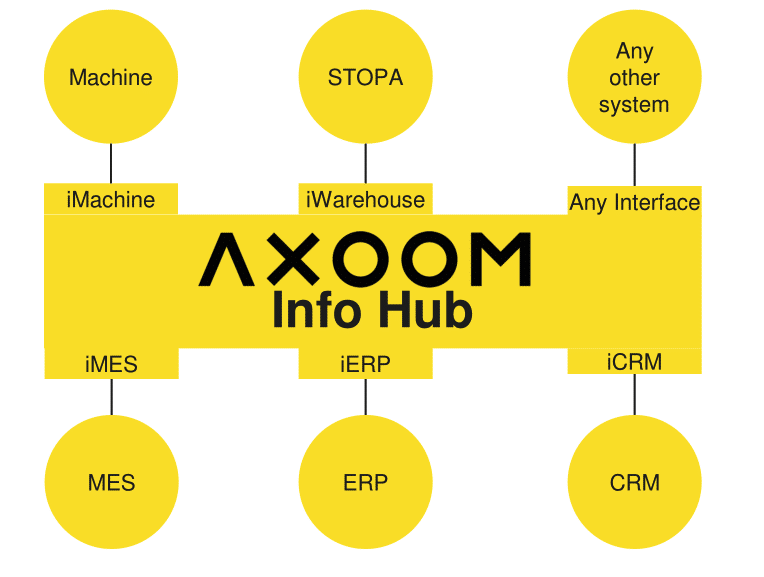
\includegraphics[width=15cm]{axoom-integration}
    \caption{AXOOM Netzwerkintegration}
    \label{Kap3:AXOOM Netzwerkintegration}
  \end{figure}
  
\clearpage

TODO - sichere Kommunikation durch AXOOM Gate - wie? Quellen? -> "Dieses basiert teilweise auf Technologien unseres Partners C-Labs und schafft eine direkte Verbindung zwischen dem Kundennetzwerk und der Cloud. Das AXOOM Gate ist in der Lage, Daten herstellerunabhängig von allen angebundenen Geräten zu sammeln, so dass diese verschlüsselt an die AXOOM Plattform gesendet und dort visualisiert und ausgewertet werden können. Besonderen Schutz bei der Datenübertragung bietet ein mehrstufiges Sicherheits- und Verschlüsselungskonzept auf Komponenten-, Transport-, Applikations- und Anwenderebene. So wird eine genaue Zugriffskontrolle innerhalb der Fabrik sowie auf die Fabrik sichergestellt, unsichere Verbindungen von und nach Außen sind ausgeschlossen."

\subsubsection{Schnittstellen}
TODO - offene Schnittstellen für Low Level
TODO - REST usw. für High Level Applications

\subsubsection{andere Kriterien}
TODO - Softwareschwachstellen, Softwarefehler 
TODO - Herstellerabhängigkeit
TODO - Kosten der Interfaceentwicklung, usw.

\section{\ac{OPC UA} Protokollanalyse}

TODO - The OPC UA specifications are layered to isolate the core design from the underlying computing technology and network transport. This allows OPC UA to be mapped to future technologies as necessary, without negating the basic design. Mappings and data encodings are described in Part 6. Three data encodings are defined:
\begin{itemize}
    \item XML/Text
    \item UA Binary
    \item JSON
\end{itemize}
In addition, several protocols are defined:
\begin{itemize}
    \item OPC UA TCP
    \item HTTPS
    \item WebSockets
\end{itemize}

TODO - ref. OPC Pt. 1

\subsection{Bedrohungsanalyse}
TODO - siehe BSI UPC UA Analyse.

\subsection{Darstellung der bzgl. IT-Sicherheit wichtigen Komponenten}


TODO - \ac{OPC UA} ist in der \ac{IEC} 62541 als offener Standard definiert und erstreckt sich über Communication- und Information Layer des \ac{RAMI4.0}, da es eine \ac{SOA} bereitstellt. 
TODO - vereint Daten und Informationsdienste. 
TODO - basiert auf IP-Netz -> Angriffsvektoren von IP und genutzten Diensten immer noch zutreffend

\begin{figure}[h]
    \centering
    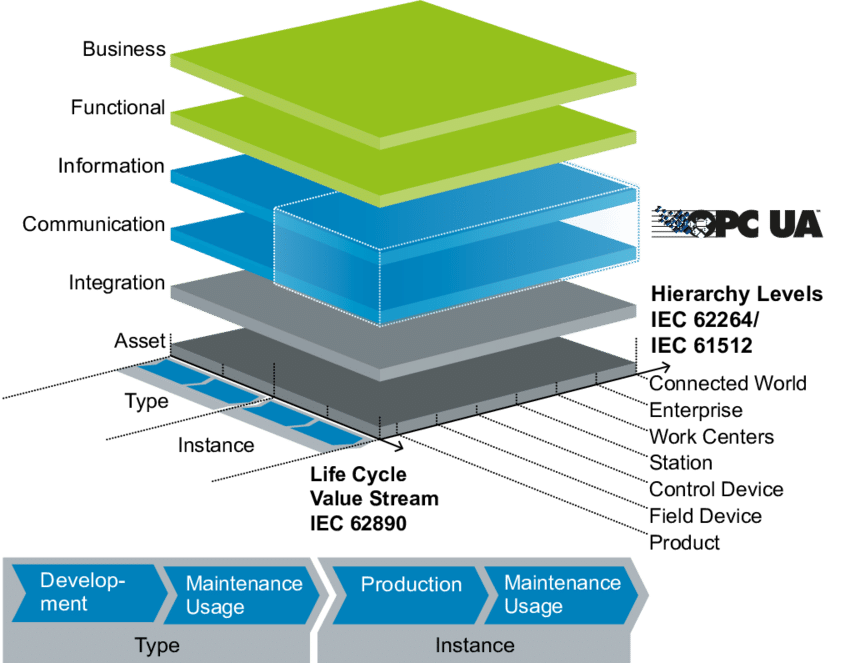
\includegraphics[width=15cm]{opcua_rami40}
    \caption{OPC UA im RAMI 4.0}
    \label{Kap3:OPC UA im RAMI 4.0}
  \end{figure}
  
\clearpage

\section{Angriffsvektoren}
\subsection{\ac{OPC UA} Spezifikation}
\subsubsection{Sicherheitslücken}
\subsubsection{Widersprüche}
\subsubsection{}

\subsection{Verschlüsselung}
\subsection{Paketversand}
\subsection{TODO}

\section{Auswertung der Ergebnisse}
\subsection{Probleme der Spezifikation}
TODO - Widersprüche in Spezifikation, sonstiges -> Syntaxfehler, usw.

\subsection{Erweiterung des Testsystems}
TODO - gefundene Schwachstellen bzw. Fehlkonfigurationen sind Grundlage der Implementierung!